%%
%% Master's survey thesis draft — ACM Computing Surveys style (acmsurvey).
%% Build: latexmk -pdf main.tex  (from this directory)
%%
\documentclass[acmsurvey,manuscript,screen,nonacm]{acmart}

\usepackage{amsmath,amssymb}
\usepackage{amsthm}
\usepackage{tikz}
\usetikzlibrary{arrows.meta,positioning,fit,calc,shapes.geometric}

\newtheorem{theorem}{Theorem}[section]
\newtheorem{proposition}[theorem]{Proposition}
\newtheorem{remark}[theorem]{Remark}

\setcopyright{none}
\copyrightyear{2026}
\acmYear{2026}

\title[Open-endedness]{Open-endedness: The Beginning of Unwritten Worlds}
\subtitle{A Survey from Genetic Algorithms to Self-Evolving Agents}
\author{Evolve Project}
\email{author@example.edu}
\affiliation{%
  \institution{Your Institution}
  \department{Your Department}
  \city{Your City}
  \country{Your Country}}

\begin{CCSXML}
<ccs2012>
<concept>
<concept_id>10010147.10010257</concept_id>
<concept_desc>Computing methodologies~Machine learning</concept_desc>
<concept_significance>500</concept_significance>
</concept>
</ccs2012>
\end{CCSXML}
\ccsdesc[500]{Computing methodologies~Machine learning}

\keywords{%
  genetic algorithms,
  evolutionary computation,
  multi-armed bandits,
  quality diversity,
  continual learning,
  self-improving AI,
  Darwin G\"odel Machine,
  ShinkaEvolve}

\begin{document}

\begin{abstract}
This survey traces a line from classical evolutionary computation and population genetics-style mathematics to modern \emph{open-ended} systems in which programs and agents evolve under stochastic evaluation.
We develop multi-armed bandits and regret minimization as the quantitative language for exploration--exploitation, connect novelty search and MAP-Elites quality diversity to stepping-stone discovery, and relate continual learning's stability--plasticity tension to non-stationary evolutionary evaluations.
We analyze two contemporary ``LLM-as-operator'' systems---ShinkaEvolve (sample-efficient program evolution) and the Darwin G\"odel Machine (empirically validated self-modifying coding agents)---and map their engineering commitments to an open-source fork (AutoImprove) that couples evolutionary loops with sandboxed evaluation.
The thesis emphasizes definitional clarity (especially for ``negative prompts'' as constraints), cites primary literature throughout, and closes with a regime-based matrix recommending algorithm families for self-evolving agents together with falsifiable predictions.
\end{abstract}

\maketitle

\section{Introduction}

\subsection{Motivation}
Biological evolution is often invoked metaphorically in optimization, but durable progress in evolutionary computation (EC) came from replacing metaphor with \emph{measurable} variation, selection, and inheritance under noise~\cite{eiben2015introduction,dejong2006evolutionary}.
The same insistence on measurement now governs systems that treat large language models (LLMs) as mutation and crossover operators over code~\cite{lange2025shinka,zhang2025darwin}.
This survey thesis asks how far one can unify three pressures---\emph{exploration} of unknown programs, \emph{exploitation} of known good parents, and \emph{safety} under incomplete verification---when the artifact being optimized is the agent itself.

\subsection{Scope and methodology}
We adopt the bounded survey protocol documented alongside this thesis (Markdown research folder): Tier~A peer-reviewed sources anchor definitions and theorems; Tier~B preprints are permitted when clearly labeled~\cite{lange2025shinka,zhang2025darwin}.
We do not attempt exhaustive enumeration of the genetic algorithms literature; instead we emphasize historically pivotal transitions (representation shifts, ES versus GA, quality diversity) that explain today's LLM-driven archives.

\subsection{Contributions of this document}
\begin{itemize}
  \item A mathematics-first reconstruction of mutation--selection processes linking Wright--Fisher intuition to evolutionary algorithms and regret minimization~\cite{ewens2004mathematical,lai1985asymptotically}.
  \item A bandit-centric explanation of exploration--exploitation with a worked finite example~\cite{auer2002finite,russo2018tutorial}.
  \item An analytic comparison of proof-gated self-modification (G\"odel machine) versus empirical validation (Darwin G\"odel Machine)~\cite{schmidhuber2007godel,zhang2025darwin}.
  \item An implementation-grounded mapping from published algorithms to the AutoImprove codebase fork of ShinkaEvolve-style evolution.
  \item A regime matrix recommending algorithm classes with explicit falsifiable predictions.
\end{itemize}

\subsection{Road map}
Section~\ref{sec:prelim} fixes notation for noisy evaluation.
Section~\ref{sec:stoch} develops Wright--Fisher drift as evolutionary intuition.
Section~\ref{sec:selection} presents Price's covariance formulation and fitness landscapes.
Section~\ref{sec:ga} surveys genetic algorithms and transitions toward code evolution.
Section~\ref{sec:bandits} develops multi-armed bandits and regret minimization.
Sections~\ref{sec:oe}--\ref{sec:rlcl} connect open-endedness, reinforcement learning, and continual learning.
Sections~\ref{sec:llm}--\ref{sec:dgm} study LLM program evolution and the Darwin G\"odel Machine.
Section~\ref{sec:neg} clarifies negative prompts as constraints.
Sections~\ref{sec:synth}--\ref{sec:auto} synthesize recommendations and repository mapping.
Section~\ref{sec:ethics} discusses evaluation hygiene and dual-use considerations.

\section{Preliminaries and noisy optimization}
\label{sec:prelim}

Let $(\Omega,\mathcal{F},\mathbb{P})$ denote a probability space carrying all randomness of evaluation (compute nondeterminism, flaky tests, LLM sampling).
A \emph{candidate} program $c$ produces a random objective observation
\begin{equation}
  Y(c) = f(c) + \varepsilon(c),
\end{equation}
where $f(c)$ is an interpretable score (e.g., mean pass rate) and $\varepsilon(c)$ aggregates measurement noise.
Evolutionary algorithms that repeatedly \emph{resample} the same candidate inherit variance both from $\varepsilon$ and from finite-population sampling~\cite{eiben2015introduction}.

\begin{remark}[Optimization versus identification]
Bandit analyses emphasize \emph{cumulative regret} while evolutionary competitions often emphasize \emph{final champion} performance.
Translating between these goals requires stating whether the training budget $T$ is large compared to mixing times of the underlying Markov chain induced by variation operators~\cite{sutton2018reinforcement}.
\end{remark}

\begin{figure}[t]
  \centering
  % Requires tikz in preamble
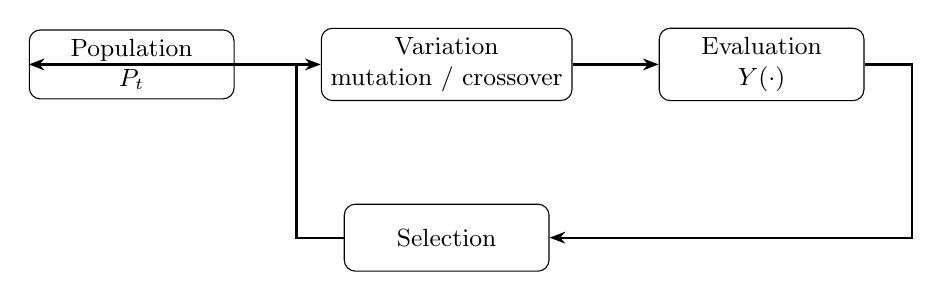
\begin{tikzpicture}[
    font=\small,
    box/.style={draw, rounded corners, minimum width=2.6cm, minimum height=0.85cm, align=center},
    arr/.style={-{Stealth[length=2mm]}, thick}
  ]
  \node[box] (pop) at (0,0) {Population\\$P_t$};
  \node[box] (var) at (4,0) {Variation\\mutation / crossover};
  \node[box] (eval) at (8,0) {Evaluation\\$Y(\cdot)$};
  \node[box] (sel) at (4,-2.2) {Selection};
  \draw[arr] (pop) -- (var);
  \draw[arr] (var) -- (eval);
  \draw[arr] (eval.east) -- ++(0.6,0) |- (sel.east);
  \draw[arr] (sel.west) -- ++(-0.6,0) |- (pop.west);
\end{tikzpicture}

  \caption{Canonical evolutionary loop with noisy fitness oracle $Y(\cdot)$.}
  \label{fig:ea-loop}
\end{figure}

Figure~\ref{fig:ea-loop} emphasizes that sandbox fidelity determines whether $Y$ approximates intended deployment fitness---a central theme when agents gain tool access~\cite{zhang2025darwin}.

\section{Random processes as evolutionary intuition}
\label{sec:stoch}

\subsection{Wright--Fisher drift}
Consider a haploid population of size $N$ with two alleles.
Let $X_t\in\{0,1/N,\dots,1\}$ denote the frequency of allele $A$.
Under neutrality (no selection differences), classical Wright--Fisher dynamics sample parents independently:
\begin{equation}
  X_{t+1} = \frac{1}{N}\,\mathrm{Binomial}(N,X_t).
\end{equation}
$(X_t)$ is a finite-state Markov chain absorbed at $0$ or $1$.
The expected frequency stays fixed, yet variance accumulates until fixation---\emph{genetic drift}~\cite{ewens2004mathematical,durrett2008probability}.

\begin{remark}[Evolutionary analogy]
Finite populations in evolutionary algorithms exhibit analogous ``allele frequency'' drift in schema proportions when selection pressure is weak relative to mutation~\cite{goldberg1989genetic}.
\end{remark}

\subsection{Branching and extinction}
Galton--Watson branching processes provide another pre-biological mental model: novel partial solutions may flourish or die before adoption~\cite{durrett2008probability}.
Quality diversity methods attempt to preserve partially successful lineages explicitly~\cite{mouret2015illuminating}.

\section{Selection mathematics: Price and landscapes}
\label{sec:selection}

\subsection{Price equation (structural)}
Price's covariance formulation decomposes change in average trait value into selection and transmission components~\cite{price1970selection,frank1995george}.
For measurable trait $z_i$ and fitness $w_i$:
\begin{equation}
  \Delta \bar{z}
  = \frac{\mathrm{Cov}(w_i,z_i)}{\bar{w}}
  + \frac{\mathbb{E}[w_i\,\Delta z_i]}{\bar{w}}.
\end{equation}
The first term captures directional selection; the second captures mutation and inheritance biases.

\subsection{Fitness landscapes}
A genotype $g\in\mathcal{G}$ maps to fitness $F(g)$.
Epistasis (non-additive interactions) creates multimodal landscapes where greedy hill climbing fails~\cite{mitchell1998introduction}.
This motivates crossover (recombination), niching, and quality diversity~\cite{deb2002fast,mouret2015illuminating}.

\subsection{Fisher's fundamental theorem: caution}
Fisher's theorem has generated extensive clarification because informal statements often misrepresent scope~\cite{fisher1930genetical}.
This thesis treats Fisher primarily as historical context and relies on formal bandit or convergence statements when precise guarantees are needed~\cite{lai1985asymptotically,auer2002finite}.

\section{Genetic algorithms: a concise historical arc}
\label{sec:ga}

Holland's framework emphasized string representations, crossover, and mutation with schema-intuitive explanations~\cite{holland1975adaptation}.
Goldberg systematized algorithm engineering practice~\cite{goldberg1989genetic}.
Parallel communities developed evolution strategies (ES) emphasizing continuous parameter spaces and self-adaptation~\cite{hansen2001completely,beyer2002evolution}.

\subsection{Modern contrasts}
\begin{itemize}
  \item \textbf{Multi-objective dominance}: NSGA-II remains a widely deployed baseline~\cite{deb2002fast}.
  \item \textbf{Distribution-based search}: CMA-ES adapts full covariance of search distributions~\cite{hansen2001completely}.
  \item \textbf{Quality diversity}: MAP-Elites archives elites across behavioral niches~\cite{mouret2015illuminating}.
\end{itemize}

\begin{figure}[t]
  \centering
  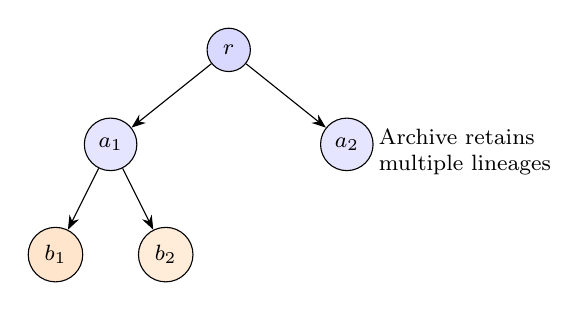
\begin{tikzpicture}[
    font=\footnotesize,
    agent/.style={circle, draw, minimum size=0.55cm},
    arr/.style={-{Stealth[length=1.8mm]}}
  ]
  \node[agent, fill=blue!15] (r) at (0,0) {$r$};
  \node[agent, fill=blue!10] (a1) at (-1.5,-1.2) {$a_1$};
  \node[agent, fill=blue!10] (a2) at (1.5,-1.2) {$a_2$};
  \node[agent, fill=orange!20] (b1) at (-2.2,-2.6) {$b_1$};
  \node[agent, fill=orange!15] (b2) at (-0.8,-2.6) {$b_2$};
  \draw[arr] (r) -- (a1);
  \draw[arr] (r) -- (a2);
  \draw[arr] (a1) -- (b1);
  \draw[arr] (a1) -- (b2);
  \node[align=left] at (3,-1.3) {Archive retains\\multiple lineages};
\end{tikzpicture}

  \caption{Toy illustration of an evolutionary archive as a tree of edits (original TikZ sketch).}
  \label{fig:archive-tree}
\end{figure}

\subsection{Transition to code evolution}
When genotypes become programs in Turing-complete languages, syntactic constraints and semantic brittleness dominate~\cite{koza1992genetic}.
LLM-based mutation operators bias proposals toward human-like code edits~\cite{lange2025shinka}.

\section{Multi-armed bandits and regret}
\label{sec:bandits}

\subsection{Stochastic $K$-armed bandits}
Arms $a\in\{1,\dots,K\}$ yield i.i.d.\ rewards in $[0,1]$ with unknown means $\mu_a$.
Let $\mu^\star=\max_a \mu_a$.
The pseudo-regret of policy $\pi$ up to horizon $T$ is
\begin{equation}
  \mathrm{Regret}_T(\pi)
  = \sum_{t=1}^{T} \bigl(\mu^\star - \mu_{A_t}\bigr),
\end{equation}
where $A_t$ is the arm pulled at time $t$~\cite{lai1985asymptotically}.

\subsection{UCB1 index policy}
Upper confidence bounds balance empirical mean estimates with optimism proportional to uncertainty~\cite{auer2002finite}.
A representative index is
\begin{equation}
  A_t \in \arg\max_{a}
  \left(
    \hat{\mu}_a(t-1) + \sqrt{\frac{2\ln t}{N_a(t-1)}}
  \right),
\end{equation}
with tie-breaking arbitrary.

\subsection{Thompson sampling}
Maintain a Bayesian posterior over reward parameters; sample one realization per round and act greedily on the sample~\cite{russo2018tutorial,agrawal2012analysis}.

\subsection{Worked micro-example}
Consider three Bernoulli arms with means $(0.50,0.55,0.80)$.
Uniform random exploration wastes pulls on clearly inferior arms; UCB reallocates pulls logarithmically toward ambiguity~\cite{auer2002finite}.

\begin{figure}[t]
  \centering
  \begin{tikzpicture}[
    font=\footnotesize,
    axis/.style={-{Stealth[length=2mm]}},
    regret/.style={thick, blue!70!black}
  ]
  \draw[axis] (0,0) -- (6.5,0) node[below] {$t$};
  \draw[axis] (0,0) -- (0,3.2) node[left] {cumulative regret};
  \draw[regret, smooth] plot coordinates {(0.4,0.15)(1,0.55)(2,1.05)(3,1.45)(4,1.85)(5,2.2)(6.2,2.65)};
  \draw[dashed, gray] (0,0) -- (6.3,2.95);
  \node[align=left] at (5.2,2.5) {\textcolor{gray}{linear if}\\\textcolor{gray}{always bad}};
\end{tikzpicture}

  \caption{Conceptual regret accumulation: suboptimal pulls contribute linearly until confidence catches structure.}
  \label{fig:bandit}
\end{figure}

\subsection{Bridge to evolutionary search}
ShinkaEvolve uses bandit-style allocation across LLM endpoints when composing mutations~\cite{lange2025shinka}.
This is an explicit algorithmic realization of exploration--exploitation beyond heuristic temperature tuning.

\section{Open-endedness and quality diversity}
\label{sec:oe}

\subsection{Novelty search}
Novelty search replaces objective fitness with novelty relative to an archive~\cite{lehman2011novelty}.
This can escape deceptive objectives when novelty correlates with discovering stepping stones.

\subsection{MAP-Elites}
MAP-Elites maintains the highest-performing solution found for each cell of a behavior descriptor grid~\cite{mouret2015illuminating}.
The resulting archive approximates a diversity--performance Pareto front under discretization~\cite{pugh2016quality}.

\subsection{POET-style co-evolution}
Coupled generation of environments and agents illustrates open-ended expansion of challenge distributions~\cite{wang2019paired}.
Recent conceptual work reframes open-endedness via sequences of learnable artifacts~\cite{hughes2024open}.

\subsection{Intrinsic motivation}
Developmental learning perspectives motivate curiosity as compression progress~\cite{oudeyer2007intrinsic}.

\begin{remark}[Descriptor design risk]
QD methods fail when descriptors omit axes along which stepping stones align~\cite{ecoffet2019go}.
\end{remark}

\section{Reinforcement learning, evolution, and continual learning}
\label{sec:rlcl}

\subsection{Where gradients win}
When simulators are differentiable or highly sample-efficient model-based RL applies, policy gradients and value-based methods dominate~\cite{sutton2018reinforcement}.
Self-play exemplifies closed-loop non-stationarity handled by curriculum emergence~\cite{silver2017mastering}.

\subsection{Where evolution wins}
Parallel rollouts and non-differentiable objectives align with evolutionary strategies~\cite{such2017deep}.
Population-based training mixes populations of RL agents with evolutionary hyperparameter adaptation~\cite{jaderberg2017population}.

\subsection{Continual learning}
Continual learning addresses catastrophic forgetting under distribution shift~\cite{kirkpatrick2017overcoming,delange2021continual,zeno2024continual}.
Non-stationary evolutionary evaluations resemble continual learning when benchmarks drift or agents self-edit evaluation harnesses~\cite{zhang2025darwin}.

\begin{remark}[Coupling concerns]
When the agent modifies its own tooling, evaluation non-stationarity may dominate biological-style drift effects from Section~\ref{sec:stoch}.
\end{remark}

\section{LLMs as mutation operators in program evolution}
\label{sec:llm}

\subsection{ShinkaEvolve}
ShinkaEvolve introduces three coupled mechanisms~\cite{lange2025shinka}:
\begin{enumerate}
  \item \textbf{Parent sampling} balancing exploration and exploitation over archived programs.
  \item \textbf{Code novelty rejection sampling} to avoid redundant proposals.
  \item \textbf{Bandit-based LLM ensemble selection} adapting operator choice online.
\end{enumerate}

\subsection{Automated design of agentic systems (ADAS)}
ADAS meta-searches code-defined agents using an archive of discoveries~\cite{hu2025adas}.
Compared with ShinkaEvolve, emphasis shifts toward discovering agent \emph{modules} rather than low-level numerical kernels~\cite{romera2024mathematical}.

\subsection{Relation to classical EC}
LLMs induce strongly biased mutation kernels concentrated on human-like edits.
Population diversity therefore depends on archive policies and stochastic sampling rather than bitwise mutation alone~\cite{lange2025shinka}.

\section{Darwin G\"odel Machine: empirical self-improvement}
\label{sec:dgm}

\subsection{Proof-gated versus benchmark-gated improvement}
Schmidhuber's G\"odel machine seeks self-modifications that are provably beneficial~\cite{schmidhuber2007godel}.
Full formal verification is rarely feasible for learned components or messy harness code~\cite{zhang2025darwin}.

\subsection{Darwin G\"odel Machine loop}
The Darwin G\"odel Machine maintains an archive of coding agents.
Parents are sampled with nonzero probability to encourage stepping stones; offspring undergo empirical evaluation on repositories~\cite{zhang2025darwin}.
Reported gains include movement from baseline scores toward stronger performance on SWE-bench variants and Polyglot~\cite{zhang2025darwin,jimenez2024swebench}.

\begin{figure}[t]
  \centering
  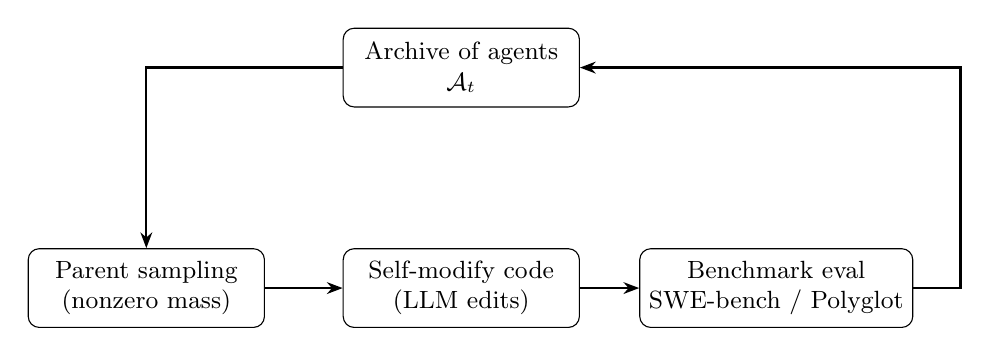
\begin{tikzpicture}[
    font=\small,
    blk/.style={draw, rounded corners, minimum width=3cm, minimum height=1cm, align=center},
    arr/.style={-{Stealth[length=2mm]}, thick}
  ]
  \node[blk] (arc) at (0,0) {Archive of agents\\$\mathcal{A}_t$};
  \node[blk] (par) at (-4,-2.8) {Parent sampling\\(nonzero mass)};
  \node[blk] (mod) at (0,-2.8) {Self-modify code\\(LLM edits)};
  \node[blk] (ev) at (4,-2.8) {Benchmark eval\\SWE-bench / Polyglot};
  \draw[arr] (arc.west) -| (par.north);
  \draw[arr] (par) -- (mod);
  \draw[arr] (mod) -- (ev);
  \draw[arr] (ev.east) -- ++(0.6,0) |- (arc.east);
\end{tikzpicture}

  \caption{Empirical self-improvement loop (original schematic inspired by published descriptions~\cite{zhang2025darwin}).}
  \label{fig:dgm}
\end{figure}

\subsection{Safety engineering}
Sandboxing and traceability mirror requirements for AutoImprove-style Docker isolation discussed in Section~\ref{sec:auto}.

\section{Negative prompts and constrained objectives}
\label{sec:neg}

\subsection{Diffusion guidance}
Classifier-free guidance interpolates conditional and unconditional score estimates~\cite{ho2022classifier}.
Negative textual prompts influence sampling through learned score corrections rather than literal logical negation.

\subsection{Language model steering}
Prompt negation in natural language does not correspond to a linear operator in latent representation spaces~\cite{raffel2020exploring}.
Constraint fulfillment often requires decoding-time filters or reinforcement from preference models.

\subsection{Evolutionary analogues}
Penalties $\lambda g(x)$, constrained MAP-Elites, and dominance constraints mirror engineering approaches for specifying forbidden behaviors~\cite{deb2002fast}.

\begin{remark}[Terminology discipline]
The phrase ``truly negative prompts'' should be defined per modality (diffusion versus autoregressive decoding versus evolutionary penalties) to avoid equivocation.
\end{remark}

\section{Synthesis: algorithm classes for self-evolving agents}
\label{sec:synth}

Table~\ref{tab:matrix} summarizes regimes discussed throughout this thesis.
Each row pairs structural assumptions with an algorithm family and a failure mode.

\begin{table}[t]
  \centering
  \caption{Regime-based recommendations (informal but actionable).}
  \label{tab:matrix}
  \small
  \begin{tabular}{p{0.22\linewidth}p{0.18\linewidth}p{0.22\linewidth}p{0.28\linewidth}}
    \hline
    Structure & Budget & Preferred class & If assumptions fail \\
    \hline
    Differentiable simulator & Medium--high & PBT / RL~\cite{jaderberg2017population} & Exploitability, instability \\
    Parallel black-box scores & High & ES / CMA-ES~\cite{hansen2001completely} & Non-stationary noise \\
    Program + tests & Medium & LLM archive evolution~\cite{lange2025shinka} & Goodharting tests \\
    Self-edit equals task & High & DGM-style validation~\cite{zhang2025darwin} & Benchmark leakage \\
    Deceptive objectives & Medium--high & MAP-Elites / novelty~\cite{mouret2015illuminating,lehman2011novelty} & Bad descriptors \\
    Distribution shift & Medium & Continual learning~\cite{zeno2024continual} & Negative transfer \\
    \hline
  \end{tabular}
\end{table}

\subsection{Falsifiable predictions}
\begin{enumerate}
  \item Bandit-style parent allocation lowers variance of best-found fitness versus truncation selection under Bernoulli evaluation noise~\cite{auer2002finite,lange2025shinka}.
  \item Archives outperform ``latest-only'' self-modification when destructive edits have positive probability~\cite{zhang2025darwin}.
  \item MAP-Elites aids deceptive tasks only when behavior descriptors align with productive stepping stones~\cite{mouret2015illuminating}.
\end{enumerate}

\section{Repository mapping: AutoImprove}
\label{sec:auto}

AutoImprove extends Shinka-style evolution with RunPod GPU compute, OpenRouter LLM access, Docker sandboxes, and a management portal (project \texttt{README.md}).
This section maps published mechanisms to Python modules.

\subsection{\texttt{autoimprove/core/evolution.py}}
\texttt{MutationOperator} wraps LLM generation and extracts executable code from model outputs.
\texttt{EvolutionEngine.\_select\_parents} ranks candidates by \texttt{combined\_score} and retains top performers---an exploitation-heavy policy complementing bandit methods in ShinkaEvolve~\cite{lange2025shinka}.
Configuration flags \texttt{archive\_enabled} and \texttt{novelty\_detection} anticipate parity with novelty rejection pipelines.

\subsection{\texttt{autoimprove/core/evaluator.py}}
\texttt{Evaluator} aggregates repeated stochastic evaluations (multiple runs, timeouts), reflecting noisy fitness observations formalized in Section~\ref{sec:prelim}.

\subsection{\texttt{autoimprove/core/orchestrator.py}}
\texttt{Orchestrator.run\_evolution} budgets API cost (\texttt{max\_api\_cost}), invokes Docker or RunPod evaluation, and tracks champion candidates---engineering correlates of sandboxed self-improvement~\cite{zhang2025darwin}.

\subsection{Gap analysis}
Instantiating Darwin G\"odel Machine-level self-referential evaluation requires coupling benchmarks directly to an agent's capacity to modify its own repository---beyond generic task evaluations wired by default configurations.

\section{Ethics, dual-use, and evaluation hygiene}
\label{sec:ethics}

\subsection{Benchmark leakage}
Coding benchmarks such as SWE-bench reward agents that reflect patterns seen during foundation model training~\cite{jimenez2024swebench}.
Surveys must separate true capability gains from memorization effects~\cite{brown2020language}.

\subsection{Sandbox boundaries}
Self-editing agents amplify classical sandbox escape risks via prompt injection into tools~\cite{zhang2025darwin}.
Docker isolation (AutoImprove) parallels stated precautions in recent empirical self-improvement studies.

\subsection{Cost transparency}
API spend and GPU rental correlate with environmental and economic impacts; reproducibility demands logged budgets akin to \texttt{max\_api\_cost} hooks.

\subsection{Dual-use}
General program synthesis can accelerate malware development; institutional review policies apply beyond technical mitigation.


\bibliographystyle{ACM-Reference-Format}
\bibliography{references}

\end{document}
